\section{xv6}

\begin{figure}[H]
    \centering
    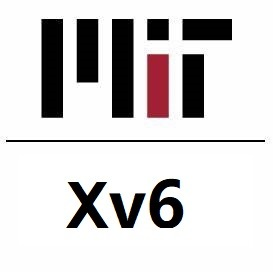
\includegraphics[width=0.35\textwidth]{figures/xv6.jpeg}
    \caption[Ícono de xv6]%
            {Ícono de xv6 \citep{pdos2016}}
    \label{fig:xv6}
\end{figure}

xv6 es un sistema operativo educativo inspirado en Unix V6, desarrollado en 2006 por el MIT para su curso de sistemas operativos. Su propósito fue proporcionar un kernel moderno y simple que sustituyera al Unix V6 original, cuya complejidad dificultaba la enseñanza. xv6 sigue de cerca la estructura de Unix V6, pero está escrito en C ANSI y se ejecuta en arquitecturas Intel multiprocesador, convirtiéndose en una herramienta práctica y comprensible para la docencia \citep{pdos2016}.  

Su arquitectura corresponde a un kernel monolítico minimalista, en el que todo el núcleo del sistema operativo se ejecuta con privilegios de kernel, sin separación en servidores independientes. xv6 incluye soporte para multiprocesadores mediante bloqueos y estructuras internas de hilos, aunque carece de controladores de red o capacidades gráficas avanzadas. Sus componentes básicos abarcan la planificación de procesos con un esquema round-robin, la gestión de memoria con paginación simple, un sistema de archivos inspirado en Unix V6 y un conjunto reducido de llamadas al sistema \citep[pp.~25]{mit2022}.  

La implementación de xv6 está escrita principalmente en C, mientras que el código de inicio y las rutinas de interrupción se desarrollan en ensamblador x86. En sus versiones más recientes, también se encuentra una adaptación para la arquitectura RISC-V, lo que amplía su aplicabilidad en contextos educativos.  

Entre los componentes principales destacan la gestión de procesos, que otorga a cada uno su propio espacio de direcciones, con un planificador round-robin y un cambio de contexto sencillo; la gestión de memoria mediante paginación básica y un asignador simple para el kernel; un sistema de archivos con inodos y directorios inspirado en Unix V6; y mecanismos elementales de sincronización como \texttt{sleep} y \texttt{wakeup}, que permiten estudiar las condiciones de carrera. Además, xv6 expone llamadas al sistema tradicionales de UNIX como \texttt{fork}, \texttt{exit}, \texttt{wait}, \texttt{open}, \texttt{read}, \texttt{write} y \texttt{close}, lo que facilita comprender la implementación exacta de estas primitivas fundamentales \citep[pp.~26--30]{mit2022}.  

xv6 se ha consolidado como una herramienta académica ampliamente utilizada en universidades para cursos de sistemas operativos. Su código fuente está disponible públicamente, y los propios autores distribuyen un libro titulado \textit{xv6: a simple, Unix-like teaching operating system}, que comenta línea por línea el código y explica tanto el funcionamiento como el diseño de sus estructuras y funciones. Gracias a su claridad y abundante documentación, xv6 se ha convertido en uno de los sistemas operativos de referencia para la enseñanza de fundamentos prácticos de diseño de kernels \citep{mit2022}.  
